\chapter{ARxCODE}
\label{chap:arxcode} 

%\endinput
\section{Especificaciones}
El ARxCODE es una aplicaci\'on para el procesamiento y an\'alisis de encuentros con riesgo de colisi\'on.\\

\subsubsection*{Funcionalidades:}
\begin{itemize}
\item Procesar la informaci\'on de los mensajes CDM.\\
\item Permitir la carga manual de la situaci\'on de encuentro.\\
\item Extraer de la web (via spacetrack) los TLE de los objetos involucrados.\\
\item .\\
\item Propagar y ajustar la posici\'on del desecho al instante del acercamiento, con su error asociado\\
\item Calcular la PoC.\\
\item Generar reportes, notificaciones y visualizaciones.\\
\end{itemize}

\section{Requerimientos}

\begin{table}
 \resizebox{\linewidth}{!}{
 \begin{tabular}{|l|l|l|}
 \hline \hline
  Req. ID & Descripci\'on & Comentario \\
  \hline \hline
  1 & Requerimientos FUNCIONALES & \\
  \hline
  ARR-010 & ARxCODE debe calcular la probabilidad de colisi\'on de un acercamiento de riesgo. & \\
  \hline
  ARR-020 & \makecell{ARxCODE debe  aceptar como inputs: un mensaje de alerta (CDM),\\ o los identificadores de NORAD de ambos objetos y\\ el tiempo de m\'aximo acercamiento (TCA) .}&\\
  \hline
  ARR-030 & \makecell{ARxCODE debe utilizar los productos orbitales de la misi\'on o realizar \\el mismo procedimiento que se aplica al desecho, a la misi\'on.}&\\
  \hline
  ARR-040 & ARxCODE debe cacular la m\'inima distancia, total y en la coordenada radial.&\\
  \hline
  ARR-050 & ARxCODE debe manipular los sistemas de referencia: TEME, TOD, VNC y RTN. &\\
  \hline
  ARR-060 & \makecell{ARxCODE debe permitir al operador/analista experto visualizar\\ el encuentro, generar reportes y notificaciones.}&\\
  \hline
  ARR-070 & \makecell{ARxCODE debe extraer el set de TLEs de los objetos involucrados \\ de los \'ultimos 15 d\'ias anteriores al TCA.}&\\
  \hline
  2 & Requerimientos de INTERFACES & \\
  \hline
  ...&...&...\\
  \hline
  3 & Requerimientos de RENDIMIENTO y/o PERFORMANCE & \\
  \hline
  ...&...&...\\
  \hline
  4 & Requerimientos de OPERACIONES & \\
  \hline
  ...&...&...\\
  \hline
  5 & Requerimientos de VALIDACI\'ON & \\
  \hline
  ...&...&...\\
  \hline
  6 & Requerimientos de DISE\~NO& \\
  \hline
  ...&...&...\\
  \hline
  7 & Requerimientos de CALIDAD& \\
  \hline
  ...&...&...\\
  \hline
  8 & Requerimientos de REUSABILIDAD & \\
  \hline
  ...&...&...\\
  \hline
  9 & Requerimientos de SEGURIDAD & \\
  \hline
  ...&...&...\\
  \hline
  10 & Requerimientos de SEGURIDAD & \\
  \hline
    ...&...&...\\
  \hline
  11 & Requerimientos de CONFIABILIDAD & \\
  \hline
  ...&...&...\\
  \hline
  12 & Requerimientos de MANTENIMIENTO & \\
  \hline
 \end{tabular}
 }
 \caption[Tabla de Requerimientos]{Tabla de especificaci\'on de requerimientos del ARxCODE}
\end{table}





\begin{itemize}
\item La aplicaci\'on detectar\'a la llegada de un CDM y ser\'a capaz de desglosarlo para extraer la informaci\'on que sea necesaria.\\
\item La aplicaci\'on identificar\'a los objetos y solicitar\'a al operador/analista experto la posici\'on precisa y la matriz varianza-covarianza en el caso de la misi\'on principal\\
\item La aplicaci\'on extraer\'a los TLEs del intervalo necesario a la p\'agina Space-Track, en el caso del desecho espacial.\\
\item La aplicaci\'on ajustar\'a la precisi\'on de la posici\'on del desecho espacial y generar\'a la matriz de varianza-covarianza para el mismo.\\
\item La aplicaci\'on calcular\'a la PoC.\\
\item La aplicaci\'on tendr\'a la capacidad de generar reportes, notificaciones y visualizaciones para facilitar la comprensi\'on y el an\'alisis del riesgo.
\item La aplicaci\'on deber\'a funcionar 7x24.
\end{itemize}

\subsection*{Requerimientos Funcionales}
\begin{itemize}
\item El sistema deber\'a funcionar en todo momento.\\
\item El software detectar\'a la llegada de un CDM y ser\'a capaz de desglozarlo para extraer la informaci\'on que sea necesaria.\\
\item El software identificar\'a los objetos y solicitar\'a informaci\'on orbital al departamento de Din\'amica Orbital en el caso de la misi\'on principal, y TLEs, en la p\'agina Space-Track, en el caso del desecho.\\
\item El software ajustar\'a la precisi\'on en la posici\'on del desecho y generar\'a la matriz de varianza-covarianza para el mismo.\\
\item El software calcular\'a la PoC.\\
\item El software generar\'a reportes, notificaciones y visualizaciones para facilitar la comprensi\'on y el an\'alisis del riesgo.
\end{itemize}



\section{Arquitectura}
El prototipo de software para el An\'alisis de Riesgo por Colisi\'on con Desechos Espaciales {\it{ARxCODE}}, ser\'a un sistema anexo a las estructuras ya existentes dentro del departamento de Din\'amica Orbital.\\
Ocupa un rol de intermediario a fin de facilitarle a un operador analista experto, herramientas para la toma de decisiones o el intercambio de informaci\'on con los organismos externos y el centro de control.\\
{\bf{Interfaces.}}\\
clases principales: TLE, EphemCODS
\subsection*{parametros globales y nomenclatura de la generacion de archivos}
Parametros:\\
\begin{itemize}
 \item satId
 \item fechaIni,fechaFin
 \item TLE/CODS
\end{itemize}

l prototipo de software para el An\'alisis de Riesgo por Colisi\'on con Desechos Espaciales {\it{ARxCODE}}, ser\'a un sistema anexo a las estructuras ya existentes dentro del departamento de Din\'amica Orbital.\\
El mismo se piensa como un intermediario capaz de: detectar los mensajes de alerta CDM provistos por el JSpOC, procesar los datos, generar mejores estimaciones para la posici\'on del desecho, solicitar datos m\'as precisos para la posici\'on de la misi\'on primaria y calcular la PoC. Todo esto a fin de facilitarle a un a un operador analista experto, herramientas para la toma de decisiones o el intercambio de informaci\'on con los organismos externos y el centro de control.\\

\begin{figure}
  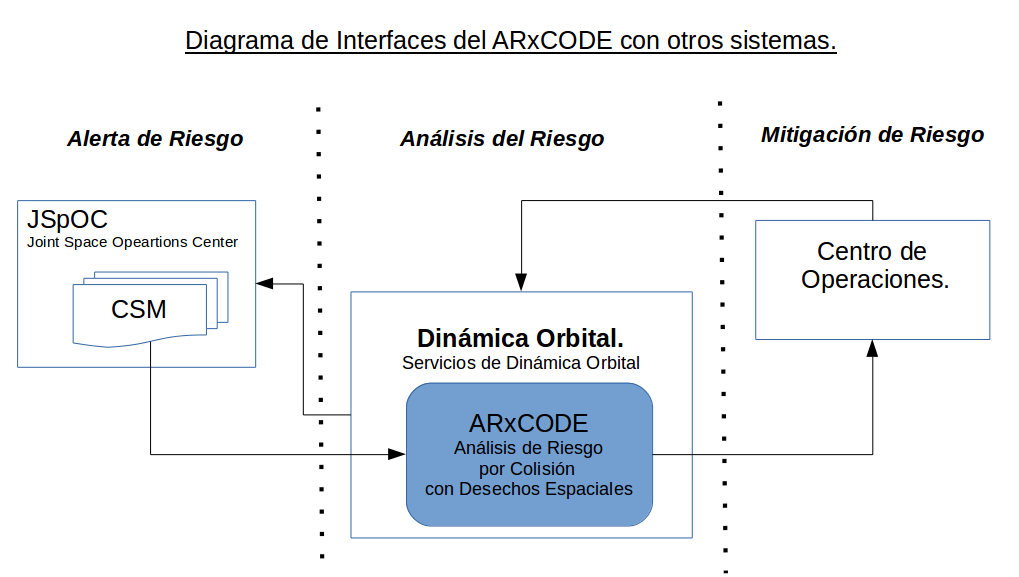
\includegraphics[width=0.8\textwidth]{imagenes/interfasessistemas}
\end{figure}

\section{Interfaces}

...ICD
\section{Entradas y Salidas}

archivos y demases

\section{Casos de Uso}

Este trabajo se pens\'o como un adicional, o un \textcolor{red}{agregado}, al software principal del departamento de din\'amica orbital. En este sentdio, no existe gran complejidad en la estrucutura del prototipo, ya que su valor, radica en la correcta implementaci\'on de los algoritmos que procesan la informaci\'on del encuentro.\\
Identificamos dos clases de uso Fig. \ref{fig:casosuso} :\\
\begin{itemize}
 \item {\it{Procesar Encuentro}}: que nuclea el procesamiento vertebral de ARxCODE
 \item {\it{Ver informes de encuentros anteriores}}: ofrece encuentros anteriores.
\end{itemize}

\begin{figure}[h!]
  \centering
  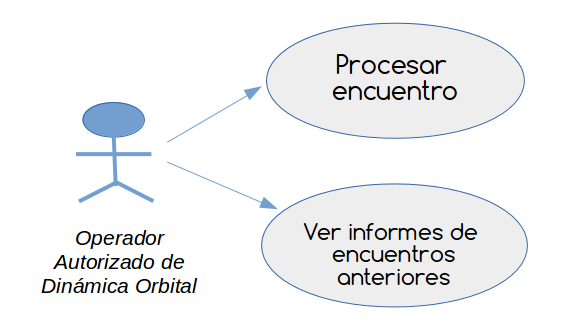
\includegraphics[width=.5\textwidth]{imagenes/casosUsos}
  \label{fig:casosuso}
  \caption{Casos de Uso de ARxCODE}
\end{figure}


 \begin{table}[h]
\centering
\resizebox{18cm}{!}{
\begin{tabular}[c]{|l|l|}
\hline
\bf{Nombre}  &    \it{Procesar Encuentro}\\
\hline
Actor  &    Operador de Din\'amica Orbital con Autorizaci\'on\\
\hline
\multirow{ 3}{*}{Prop\'osito} & Calcular la probabilidad de colisi\'on, la m\'inima distancia total\\
& y m\'inima distancia en la coordenada radial, para poder hacer un an\'alisis\\
& de la situaci\'on de encuentro.\\
\hline
\multirow{ 4}{*}{Resumen}& Procesa la ingesta de datos de un encuentro, (CDMs o ingreso manual)\\
&  y calcula los par\'ametros de la situaci\'on de riesgo:\\
& m\'inima distancia total, m\'inima distancia en la coordenada radial y probabilidad de colisi\'on.\\
& Realiza gr\'aficos e informes.\\
\hline
Requerimientos  &    \\
\hline
Precondiciones  &  El operador debe estar registrado en la p\'agina space-track de NORAD.  \\
\hline
\multirow{ 3}{*}{Flujo Principal} & 1 - El operador selecciona un archivo CDM \\
& 2 - El operador oprime el bot\'on {\it{Track}} para visualizar el encuentro proyectado en la superficie terrestre (opcional)\\
& 3 - El operador oprime el bot\'on para genera un informe (opcional)\\
\hline
\multirow{ 3}{*}{Flujo Alternativo} & 1 - El operador ingresa los n\'umeros de identificaci\'on de los objetos (NORAD\_ID) \\
& 2 - El operador ingresa la fecha y hora del m\'aximo acercamiento (TCA)\\
& 3 - El operador oprime el bot\'on {\it{Procesar}} para procesar el encuentro\\
\hline
\end{tabular}}
\caption[Caso de Uso: Procesar Encuentro]{Tabla con la descripci\'on del caso de uso: \it{Procesar Encuentro}}
\label{tab:usoproceso}
\end{table}

\subsection*{Preprocesamiento de los Datos de Misi\'on de CODS}
Para este trabajo CONAE nos facilit\'o el acceso a los datos orbitales de la misi\'on SAC-D.
Los datos se ecuentran montados en un servidor que contiene la informaci\'on organizada en archivos con formato ASCII, distribuidos en distintas carpetas seg\'un su clasificaci\'on.\\
Para la comparaci\'on que proponemos, solicitamos acceso a los archivos de efem\'erides orbitales ORBEPHEM, que ofrecen posiciones y velocidades tabuladas cada un minuto, en el Sistema de Referencia TOD (True of Date), en coordenadas cartesianas.

\subsection*{ORBEPHEM}
Estos productos son generados luego de un post procesamiento que incluye una propagaci\'on ajustada por una determinaci\'on orbital. 
Cada archivo contiene un listado cronol\'ogicamente tabulado de posiciones y velocidades, dentro de un periodo de casi 3 d\'ias. ( doc\_interfaces)

La nomenclatura de los mismos respeta el siguiente formato:\\
\begin{verbatim}
 CODS_YYYYMMDD_HHMMSS_SACD_ORBEPHEM_TOD_XYZ_O.TXT
 
 Donde:
  CODS = Identifica el Servicio dentro del CUSS que presta la información.
  YYYYMMDD_HHMMSS = epoca de generación del dato.
  SACD = Identificación del Satélite.
  ORBEPHEM = Tipo de Dato, Efeméride Orbital (procesada a posteriori)
  TOD = Sistema de Referencia True of Date.
  XYZ = Tipo de efeméride, cartesiana.
  O = Operacional. 
\end{verbatim}


\subsection*{Archivos Utilizados}
Si bien la nomenclatura de los archivos respeta una estructura, s\'olo se indica en el nombre, la fecha de generaci\'on de los datos y no puede desprenderse del mismo cu\'al es la \'epoca final e inicial de cada archivo, y no existe un registro del los gaps de datos ausentes. A su vez, las \'epocas contempladas en cada uno de ellos no está homogeneizada. Es decir, la fecha y hora inicial y final de cada registro es diferente para cada archivo.\\
Dada esta organizaci\'on, para el punto tres del procedimiento, referente a la localizaci\'on del archivo necesario para la comparaci\'on, la b\'usqueda se realiza de la siguiente manera:\\
Localizamos en primer lugar el archivo cuyo nombre coincide con la fecha de la \'epoca del TLE primario.
Como una misma fecha se encuentra en m\'as de un archivo, buscamos el archivo que contenga esa fecha y que adem\'as sea el m\'as actualizado de todos. Para ello, además del archivo cuyo nombre contiene la fecha del TLE primario, se enlistan los siguientes dos archivos y se ordenan en orden decreciente, de manera que el primer lugar de la lista lo ocupe el \'ultimo de los archivos seleccionados. Finalmente se comienza el proceso iterativo de abrir los archivos, evaluar el contenido y ver si se encuentran los dos registros que encierren la \'epoca del TLE.
Una vez que se encuentran las l\'ineas de efem\'erides que contienen la \'epoca de inter\'es se interpola, y se termina la iteraci\'on.

\noindent
Cantidad TOTAL de archivos $=  1454$\\
Cantidad media de resgistros por archivo $=  2688$\\
Archivo con el mayor n\'umero de registros $=  3042$\\
Archivo con el menor n\'umero de registros $=  142$\\

Im\'agenes comparativas entre los dos m\'etodos:\\
{\bf{Intervalo Estable}}\\
% \begin{figure}[htbp]
%  \centering
%   \subfigure[Procesamiento de Datos de Mision]{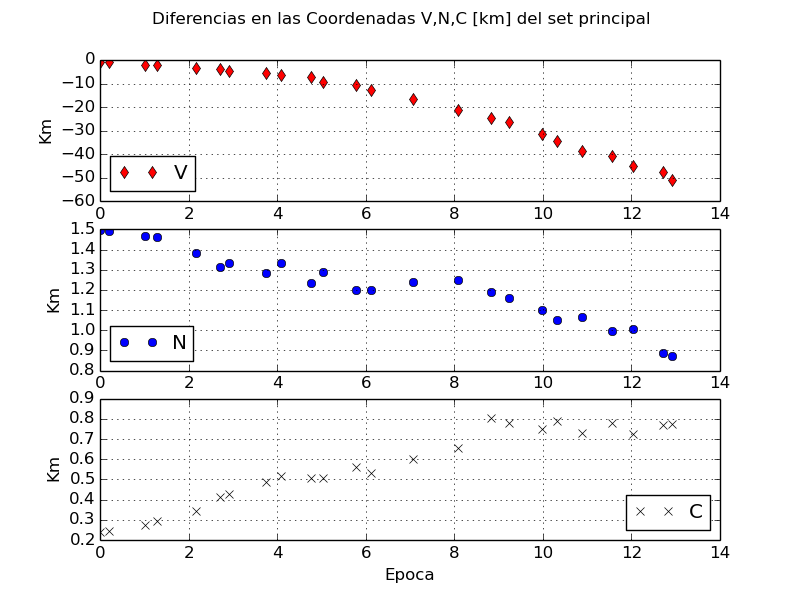
\includegraphics[width=0.46\linewidth]{imagenes/CODSsetPri37673U20120414}}
%   \subfigure[Procesamiento de TLEs]{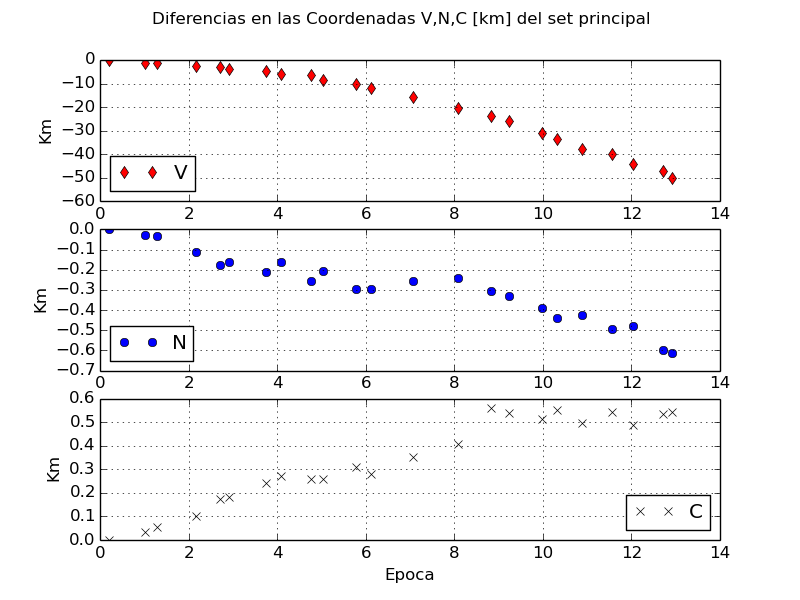
\includegraphics[width=0.46\linewidth]{imagenes/TLEsetPri3767320120414}}
%  \caption{Resultado del m\'etodo de Pair-Wise Differencing considerando TLEs y Datos de Misi\'on.}
%  \label{fig:test}
% \end{figure}

\begin{verbatim}
------------------------------------------------------------------------
DIFERENCIAS:
-------------------------------------------------------------------------
dv = -0.773155546799
dn = 1.49461651773
dc = 0.241331995666
-------------------------------------------------------------------------
\end{verbatim}

{\bf{Intervalo de Maniobra}}

% \begin{figure}[htbp]
%  \centering
%   \subfigure[Procesamiento de Datos de Mision]{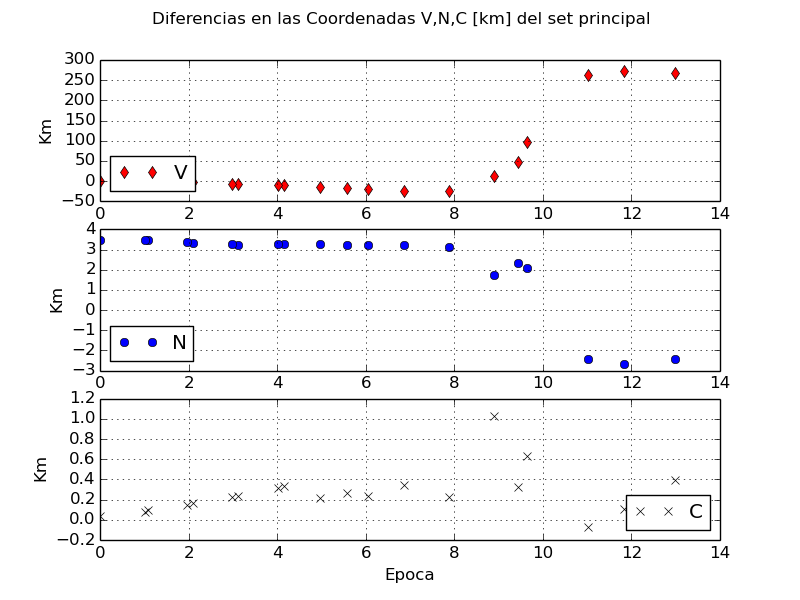
\includegraphics[width=0.46\linewidth]{imagenes/CODSsetPri37673U20120314}}
%   \subfigure[Procesamiento de TLEs]{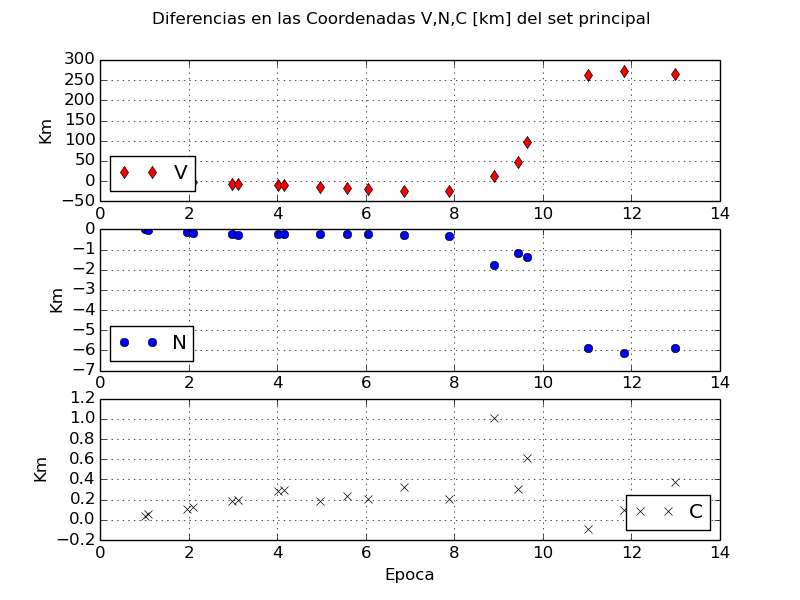
\includegraphics[width=0.46\linewidth]{imagenes/TLEsetPri3767320120314}}
%  \caption{Resultado del m\'etodo de Pair-Wise Differencing considerando TLEs y Datos de Misi\'on.}
%  \label{fig:test}
% \end{figure}

\begin{verbatim}
\begin{verbatim}
------------------------------------------------------------------------
DIFERENCIAS:
-------------------------------------------------------------------------
dv = 0.263912038422
dn = 3.47362819854
dc = 0.0366536642778
-------------------------------------------------------------------------
\end{verbatim}

\subsubsection*{Ajuste Polyfit}

{\bf{numpy.polynomial.polynomial.polyfit}}

Returns:	

coef : ndarray, shape (deg + 1,) or (deg + 1, K)

    Polynomial coefficients ordered from low to high. If y was 2-D, the coefficients in column k of coef represent the polynomial fit to the data in y‘s k-th column.

residuals, rank, singular\_values, rcond : list

    These values are only returned if full = True

    resid – sum of squared residuals of the least squares fit rank – the numerical rank of the scaled Vandermonde matrix sv – singular values of the scaled Vandermonde matrix rcond – value of rcond.

    For more details, see linalg.lstsq.

\begin{verbatim}
Procesando datos TLE...
++++++++++++GRADO 2++++++++++++++++++
[array([-1.89669503, -0.73973919, -0.06103362])]
[[array([ 31434.82805686]), 3, array([ 1.68700379,  0.388,  0.056]), 5.1292e-14]]
++++++++++++GRADO 1++++++++++++++++++
[array([ 1.93247211, -1.78532883])]
[[array([ 31556.32886285]), 2, array([ 1.393,  0.24171176]), 5.1292e-14],]
\end{verbatim}

% \section{Graficos LAGEOS 8820}
% 
% \begin{figure}[H]
%  \centering
% \begin{subfigure}%{0.5\textwidth}
%   \centering
%   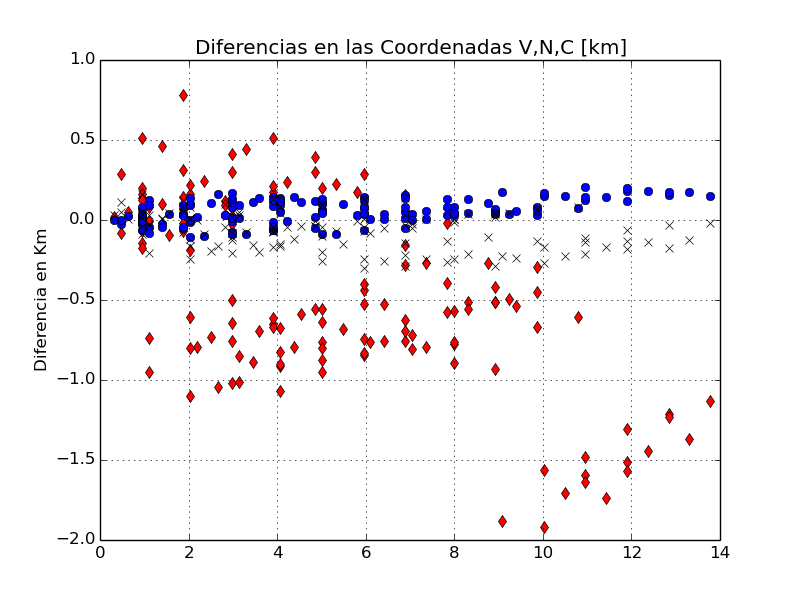
\includegraphics[width=0.7\linewidth]{imagenes/difTot8820.png}
%   \caption{A subfigure}
%   \label{fig:sub1}
% \end{subfigure}%
% \begin{subfigure}%{0.5\textwidth}
%   \centering
%   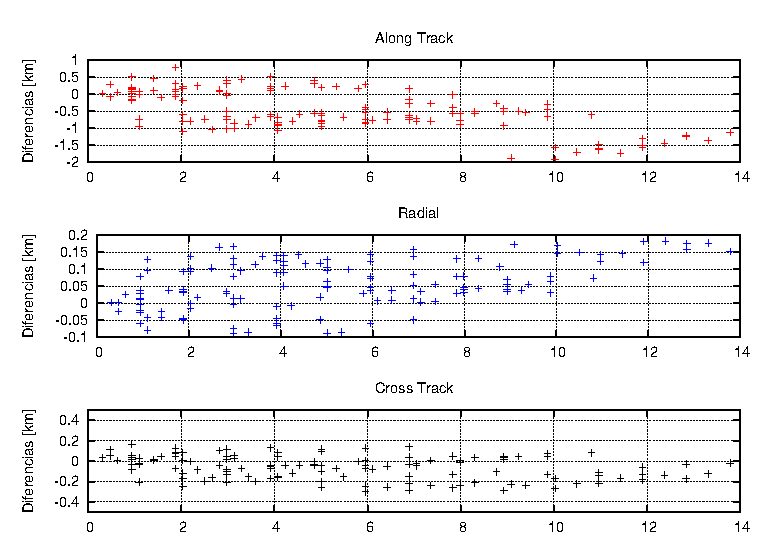
\includegraphics[width=0.7\linewidth]{imagenes/vncmultiplot}
%   \caption{A subfigure}
%   \label{fig:sub2}
% \end{subfigure}
% \caption{A figure with two subfigures}
% \label{fig:test}
% \end{figure}


\section*{Diferencias}
A partir de los datos de Misión. 

\begin{figure}[!h]
  \centering
  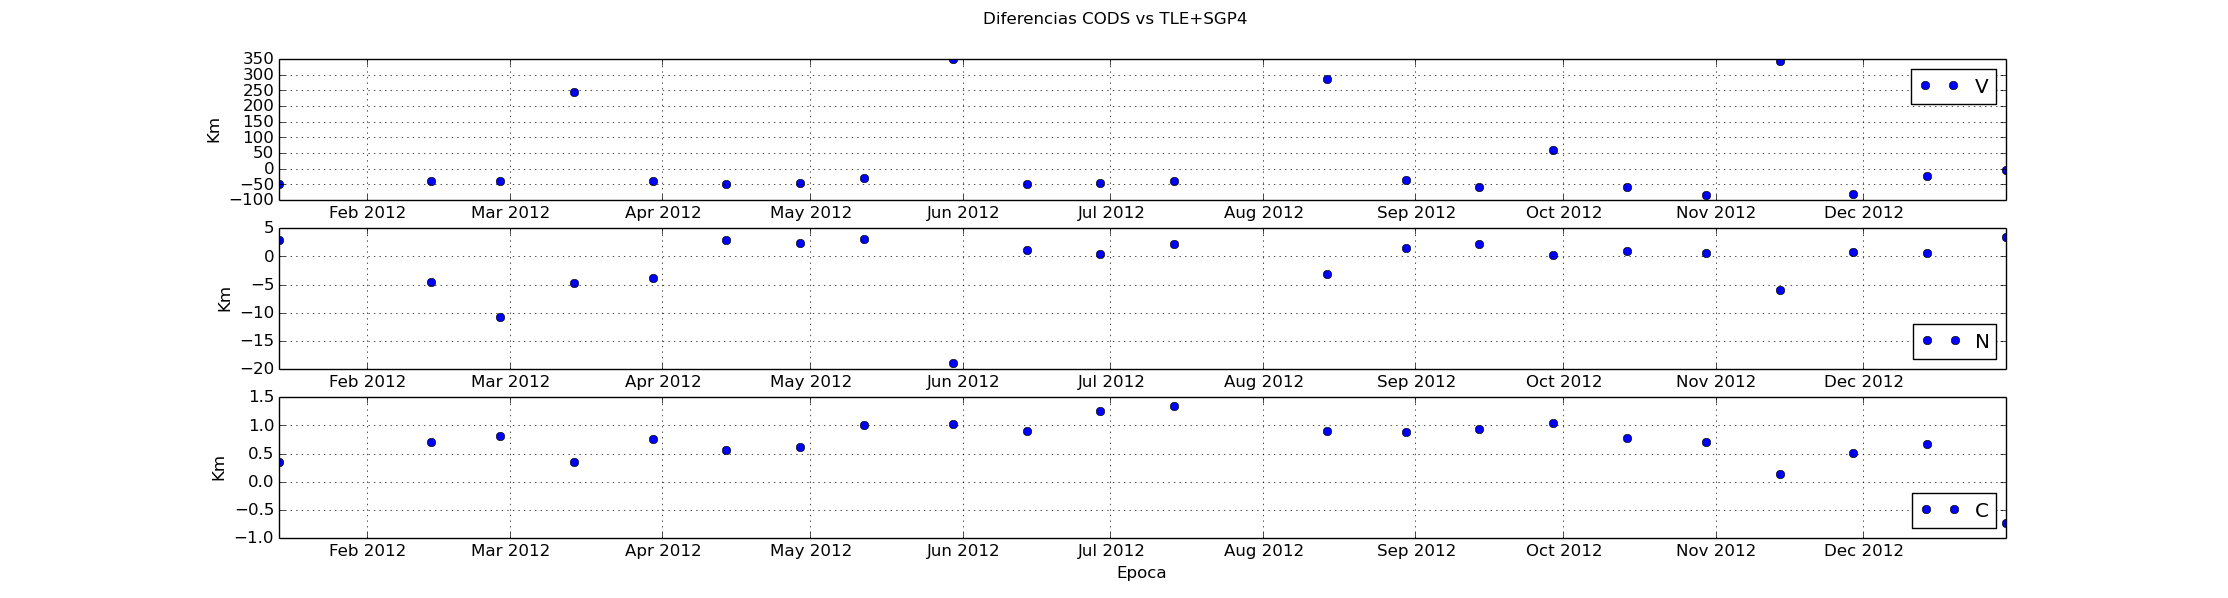
\includegraphics[width=\textwidth]{imagenes/sesgoTLE}
\end{figure}

\begin{itemize}
 \item Revisar escritura sobre datos CODS.
 \item Comparar defasaje inicial con defasaje de TLE respecto de GPS. (ver tendencias - empezar a diagramar los apédices)
 \item Comparar errores lineal vs cuadr\'atico.
\end{itemize}

\section{C\'alculo de la Probabilidad de Colisi\'on}
metodo ARxCODE ¿?¿?
% \begin{figure}[!h]
% \centering
%  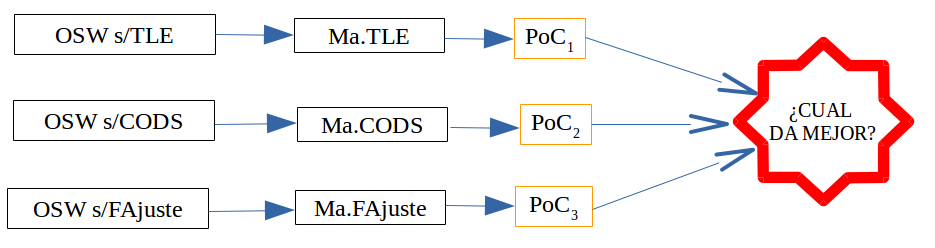
\includegraphics[width=0.5\textwidth]{imagenes/metodoARxCODE}
%  \caption{Metodolog\'ia Propuesta}
%  \label{fig:metodoARxCODE}
% \end{figure}
